\documentclass[12pt]{beamer}

\usepackage[english]{babel}
\usepackage[utf8]{inputenc}
\usepackage[T1]{fontenc}
\usepackage{amsmath,amsfonts,amsthm,amssymb}
\usepackage{mysymbols}
\usepackage{graphicx}
\usepackage{tikz}
\usetikzlibrary{positioning}
\usetikzlibrary{calc}
\usetikzlibrary{decorations.pathreplacing}
\usetikzlibrary{matrix}
\usetikzlibrary{intersections}
\usetikzlibrary{backgrounds}
\usetikzlibrary{fit}
\usetikzlibrary{arrows}
\usepackage{algorithm}
\usepackage{algorithmic}

\mode<presentation>{
  \usetheme{uvsq}
}
% For graying out overlays
\setbeamercovered{transparent}

\title{Algorithms for $\clot\FF_p$}

\author[Luca De Feo]{Luca De Feo\inst{1}\\
  joint work with Javad Doliskani\inst{2} and Éric Schost\inst{2}}

\institute[UVSQ]{\inst{1}Université de Versailles -- Saint-Quentin-en-Yvelines\\
  \inst{2}University of Western Ontario}

\date[UPMC, Sep 12, 2013]{Université Pierre et Marie Curie, Séminaire SALSA, September 12, 2013}

\begin{document}

\setbeamertemplate{navigation symbols}{}
\frame[plain]{\titlepage}

%% 

\begin{frame}
  \frametitle{What does $\clot\FF_p$ look like?}
  
  \tikzset{
    dotstyle/.style={circle, inner sep = 1.2pt, outer sep = 4pt, fill = gray},
    edgetower/.style={thick},
    edgecomp/.style={thick, lightgray}
  }
  \begin{tikzpicture} [scale = 0.8] %, every node/.style={inner sep = 2pt, scale=0.8}]
    \coordinate (T2) at (-2, 0.5);
    \node (Fp) at (0, 0) {$\FF_p$};
    \node (Fp2) at ($(Fp) + (T2)$) {$\FF_{p^2}$};
    \node (Fp4) at ($(Fp2) + (T2)$) {$\FF_{p^4}$};
    \node (Fp2l) at ($(Fp4) + (T2)$) {$\FF_p^{(2)}$};
    % ---------------------
    \coordinate (T3) at (-0.7, 2);
    \node (Fp3) at ($(Fp) + (T3)$) {$\FF_{p^3}$};
    \node (Fp9) at ($(Fp3) + (T3)$) {$\FF_{p^9}$};
    \node (Fp3l) at ($(Fp9) + (T3)$) {$\FF_p^{(3)}$};
    % ---------------------
    \coordinate (T5) at (0.7, 2);
    \node (Fp5) at ($(Fp) + (T5)$) {$\FF_{p^5}$};
    \node (Fp25) at ($(Fp5) + (T5)$) {$\FF_{p^{25}}$};
    \node (Fp5l) at ($(Fp25) + (T5)$) {$\FF_p^{(5)}$};
    % ---------------------
    \coordinate (Tl) at (2, 1);
    \node[blue] (Fpl) at ($(Fp) + (Tl)$) {$\FF_{p^\ell}$};
    \node[blue] (Fpl2) at ($(Fpl) + (Tl)$) {$\FF_{p^{\ell^2}}$};
    \node[blue] (Fpll) at ($(Fpl2) + (Tl)$) {$\FF_p^{(\ell)}$};
    % ---------------------
    \node[dotstyle] (dot1) at ($(Fp2) + (Fp3) - (Fp)$) {};
    \node[dotstyle] (dot2) at ($(Fp4) + (dot1) - (Fp2)$) {};
    \node[dotstyle] (dot3) at ($(Fp2) + (Fp5) - (Fp)$) {};
    \node[dotstyle] (dot4) at ($(Fp3) + (Fp5) - (Fp)$) {};
    \node[dotstyle] (dot5) at ($(Fp3) + (Fpl) - (Fp)$) {};
    \node[dotstyle] (dot6) at ($(Fp5) + (Fpl) - (Fp)$) {};
    % ---------------------
    \draw 
    (Fp) 
    edge[edgetower] (Fp2)
    edge[edgetower] (Fp3)
    edge[edgetower] (Fp5)
    edge[edgetower, blue] (Fpl)
    (Fp2)
    edge[edgetower] (Fp4)
    edge[edgecomp] (dot1)
    (Fp4)
    edge[edgetower, dotted] (Fp2l)
    edge[edgecomp] (dot2)
    (dot1)
    edge[edgecomp] (dot2)
    (Fp3)
    edge[edgetower] (Fp9)
    edge[edgecomp] (dot1)
    edge[edgecomp] (dot4)
    (Fp9)
    edge[edgetower, dotted] (Fp3l)
    (Fp5)
    edge[edgetower] (Fp25)
    edge[edgecomp] (dot4)
    edge[edgecomp] (dot6)
    (Fp25)
    edge[edgetower, dotted] (Fp5l)
    (Fpl)
    edge[edgetower, blue] (Fpl2)
    edge[edgecomp] (dot6)
    (Fpl2)
    edge[edgetower, blue, dotted] (Fpll)
    (dot3)
    edge[edgecomp] (Fp2)
    edge[edgecomp] (Fp5)
    (dot5)
    edge[edgecomp] (Fp3)
    edge[edgecomp] (Fpl);
    % ---------------------
    \draw [xshift = 4.5cm] node [right, text width = 2.5cm, 
    rounded corners, fill=red!10, inner sep = 1mm]{
      \small
      \mbox{$\displaystyle\FF_p^{(\ell)} = \bigcup_{i\ge 0}\FF_{p^{\ell^i}},$}\\
      \smallskip
      \mbox{$\displaystyle\clot\FF_p \cong \bigotimes_{\ell\text{ prime}} \FF_p^{(\ell)}$}
    };
  \end{tikzpicture}
\end{frame}

%% 

\begin{frame}
  \frametitle{In software}

  \begin{definition}[Compatible lattice]
    \begin{itemize}
    \item A collection of finite fields $\FF_{p^n}$ for any $n\ge 1$;
    \item A collection of morphisms $\FF_{p^m} \hookrightarrow \FF_{p^n}$ whenever $m|n$.
    \end{itemize}
  \end{definition}

  \begin{block}{Fact}
    Given a lattice, any element of $\clot\FF_p$ can be represented as
    an element of a finite field in the lattice.
  \end{block}

  \begin{block}{(Lenstra, De Smit \& Lenstra) \hfill\alert{$\Omega(n^3)$}}
    There exist a determinisitic algorithm that constructs a
    compatible lattice in time polynomial in $\log p$ and $n$, where
    $n$ is the degree of the largest computed extension of $\FF_p$.
  \end{block}
\end{frame}

%% 

\begin{frame}
  
\begin{tikzpicture}
    \node [rectangle, line width=0.7pt, draw=red!50] (abstract) { \hspace*{0.03\textwidth}%
      \begin{minipage}{0.92\textwidth}
        \vspace*{3mm}
        \begin{itemize}
        \item \emph{Efficient} construction of lattices,
        \item \emph{Efficient} field operations.
        \end{itemize}
      \end{minipage}\hspace*{0.03\textwidth}
    };%
    \node[right=0.03\textwidth,
    rectangle,
    line width=0.5pt,
    rounded corners=2pt,
    draw=red,
    fill=blue!20,
    inner xsep=3pt, inner ysep=3pt] at (abstract.north west) {\it\bfseries Our interest};
  \end{tikzpicture}
  
  \vspace*{3mm}
  \textbf{Goals}:
  \begin{itemize}
  \item Constructing fields:
    \begin{itemize}
    \item Build irreducible polynomials in quasi-linear time.
    \end{itemize}
  \item Describing embeddings:
    \begin{itemize}
    \item Quasi-linear time and memory in the degree of the extension.
    \end{itemize}
  \item Evaluating embeddings:
    \begin{itemize}
    \item Replace linear algebra by polynomial arithmetic.
    \end{itemize}
  \end{itemize}
  
  \vspace*{3mm}
  \textbf{Application examples}:
  \begin{itemize}
  \item General: finite field arithmetic, unramified extensions of $\QQ_p$.
  \item Computing isogenies between elliptic curves, DF, 2011.
  \item Point-counting in genus 2, Gaudry and Schost, 2012.
  \end{itemize}
  
\end{frame}

%% 

\begin{frame}
  \frametitle{Known constructions}

  \begin{block}{Construct fields arbitrarily + compute embeddings}
    \begin{itemize}
    \item Describe the embeddings
      \begin{itemize}
      \item Factor minimal polynomials,
      \item Allombert's isomorphism algorithm (in Pari?).
      \item Rains' isomorphism algorithm (unpublished, in Magma),
      \end{itemize}
    \item Evaluate the embeddings
      \begin{itemize}
      \item Linear algebra,
      \item Map generators (polynomial arithmetic).
      \end{itemize}
    \end{itemize}
  \end{block}
  
  \begin{block}{Construct fields defined by special polynomials}
    \begin{itemize}
    \item (pseudo)-Conway polynomials,
    \item Cyclotomy theory (De Smit \& Lenstra and generalizations),
    \item Fancy (and still limited) constructions (this talk).
    \end{itemize}
  \end{block}
\end{frame}

%% 

\section{Towers}
\frame{\sectionpage}

%% 

\begin{frame}
  \frametitle{Univariate vs. Multivariate}

  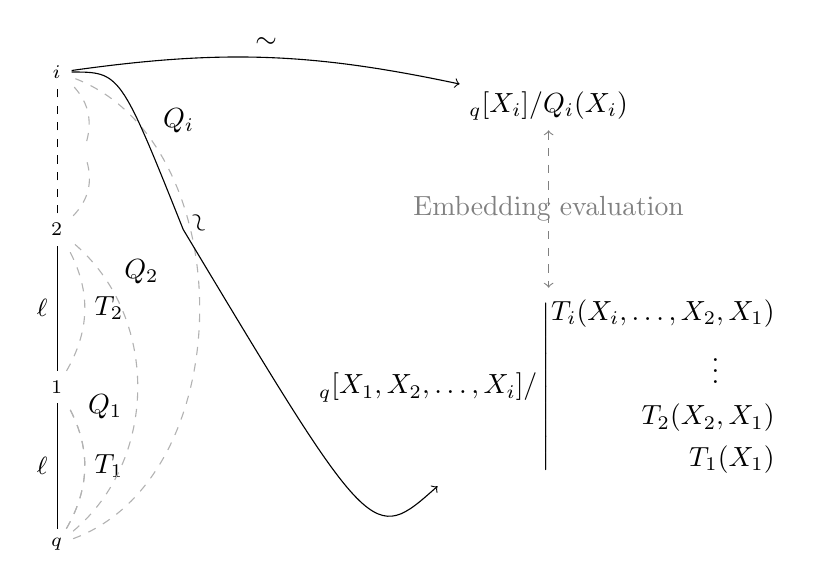
\begin{tikzpicture}
    \begin{scope}[node distance=2cm]
      \node (F0) {$\FF_q$};
      \node[above of = F0] (F1) {$\KK_1$};
      \node[above of = F1] (F2) {$\KK_2$};
      \node[above of = F2] (Fi) {$\KK_i$};
      \draw (F0) -- node[auto]{\small$\ell$} (F1) -- node[auto]{\small$\ell$} (F2);
      \draw[dashed] (F2) -- (Fi);
      \visible<2>{
        \path (F2) to[bend right] node (F2i){} (Fi);
        \draw[dashed,color=black!30,bend right,every node/.style={auto,swap,color=black}]
        (F0) edge node {$T_1$} (F1)
        (F1) edge node {$T_2$} (F2)
        (F2) edge (F2i)
        (F2i) edge (Fi);
      }
      \visible<3>{
        \draw[dashed,color=black!30,auto,swap,pos=0.8]
        (F0) edge[bend right=30] node[color=black] {$Q_1$} (F1)
        (F0) edge[bend right=50] node[color=black] {$Q_2$} (F2)
        (F0) edge[bend right=70] node[color=black] {$Q_i$} (Fi);
      }
    \end{scope}
    %%%%%%%%%%%%%%%%%%%%%%% 
    \uncover<2->{
      \node[right=3cm of F1] (T) {
        $\FF_q[X_1,X_2,\dots,X_i] /
        \left|\begin{aligned}
            T_i(X_i, \dots, X_2, X_1)\\
            \vdots\qquad\\
            T_2(X_2, X_1)\\
            T_1(X_1)
          \end{aligned}\right.
        $
      };
    }
    \visible<2>{
      \draw[->] (Fi) .. controls +(0.8cm,0cm) .. +(1.6cm,-2cm)
      node[pos=1,auto,sloped] {$\sim$}
      .. controls +(2.4cm,-4cm) .. (T)  ;
    }
    \uncover<3->{
      \node[above = 2cm of T] (Q) {
        $\FF_q[X_i] / Q_i(X_i)$
      };
    }
    \visible<3->{
      \draw[<->,dashed,color=black!50] 
      (Q) edge node {Embedding evaluation} (T);
      \draw[->] (Fi) to[bend left=10] node[auto,sloped] {$\sim$} (Q);
    }
  \end{tikzpicture}
\end{frame}

% ###################################################

\begin{frame}
  \frametitle{Summary of Main Results}
  \footnotesize

  \vspace{-2mm}

  \begin{block}{Previous work}
    \begin{itemize}
    \item Artin-Schreier (Cantor, Couveignes, DF \& Schost): $q$ fixed, \alert{$\ell=p$} small;
    \item Dyadic towers (Doliskani \& Schost): $q$ fixed, \alert{$\ell=2$};
    \item \alert{$\tildO(\ell^{i+c})$} operations in $\FF_q$, $c\in\{1,2\}$.
    \end{itemize}
  \end{block}  

  \vspace{-2mm}

  \begin{block}{This work: objective}
    \begin{itemize}
    \item $q$ fixed, $\ell$ small: \alert{$\tildO(\ell^i)$} operations in $\FF_q$;
    \item Limit additional factors in $\ell$ and $q$ as much as possible.
    \end{itemize}
  \end{block}
  
  \vspace{-2mm}

  \resizebox{0.93\textwidth}{!}{
    \begin{minipage}{\textwidth}
      \[
      \begin{array}{c|cccc}
        \text{Condition} & \text{\bf Initialization} & \mathbf{Q_i, T_i} & \text{\bf Embedding eval.}\\
        \hline \hline
        q = 1 \bmod \ell & O(1)  & O(\ell^i) & O(\ell^i) \\
        q = -1 \bmod \ell & O(1) & O(\ell^i) & O(\Mult(\ell^i) \log(\ell^i)) \\
        - & O (\ell^2) & O(\Mult(\ell^{i+1})\Mult(\ell)\log(\ell^i)^2) & O( \Mult(\ell^{i+1})\Mult(\ell)\log(\ell^i))\\
        4\ell \le q^{1 / 4} & \tildO(\ell^3) \text{~(bit)}  & O(\Mult(\ell^i)\log(\ell^i)) & O(\Mult(\ell^i) \log(\ell^i)) \\
        4\ell \le q^{1 / 4} & \tildO(\Mult(\ell)) & O(\Mult(\ell^i) \log(\ell^i)) & O(\Mult(\ell^i) \log(\ell^i)) \vspace{-0.5cm}
      \end{array}
      \]
    \end{minipage}
  }
\end{frame}

% **********************************************************
% **********************************************************

\section{Quasi-cyclotomic towers}

\begin{frame}
  \frametitle{\insertsection 
    \\{\small\normalfont\footnotesize \color{black} 
      (inspired by Shoup, Allombert, De Smit and Lenstra)}}
  
  \begin{columns}
    \begin{column}{0.65\textwidth}
      \begin{center}
        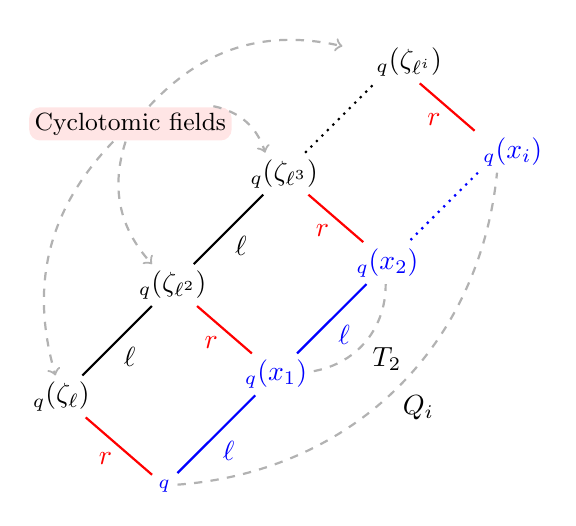
\begin{tikzpicture}[thick, node distance=2cm, inner sep = 2pt]
          \node[blue] (Q) {$\FF_q$};
          \node (Q0) [above left = 1cm of Q]{$\FF_q(\zeta_\ell)$};
          \node[blue] (K1) [above right of=Q]{$\FF_q(x_1)$};
          \node (Q1) [above right of=Q0]{$\FF_q(\zeta_{\ell^2})$};
          \node[blue] (K2)[above right of=K1]{$\FF_q(x_2)$};
          \node (Q2) [above right of=Q1]{$\FF_q(\zeta_{\ell^3})$};
          \node[blue] (Koo)[above right of=K2]{$\quad \FF_q(x_i)$};
          \node (Qoo) [above right of=Q2]{$\quad\FF_q(\zeta_{\ell^i})$};
          % --------------------------
          \draw (Q) edge[red] node[auto]{$r$} (Q0)
          edge[blue] node[auto,swap]{$\ell$} (K1)
          (K1) edge[red] node[red, auto] {$r$} (Q1)
          edge[blue] node[auto,swap]{$\ell$} (K2)
          (Q1) edge node[auto]{$\ell$} (Q0)
          (Q2) edge[red] node[red, auto, swap]{$r$} (K2)
          edge node[auto]{$\ell$} (Q1)
          edge[dotted] (Qoo)
          (Koo) edge[blue, dotted] (K2)
          edge[red] node[red, auto]{$r$} (Qoo);
          % --------------------------
          \uncover<1>{
            \node (cyclo) [above left = 2mm of Q2, fill = red!10, rounded corners, font=\small]{ Cyclotomic fields };
            \draw[dashed, ->, color = black!30] (cyclo) edge[bend right] (Q0)
            edge[bend right] (Q1)
            edge[bend left] (Q2)
            edge[bend left] (Qoo);}
          % --------------------------
          \uncover<2>{
            \draw[dashed,bend right=40,color = black!30]
            (K1) edge node[auto,swap,color=black]{$T_2$} (K2)
            (Q) edge node[auto,swap,color=black]{$Q_i$} (Koo);
          }
        \end{tikzpicture}
      \end{center}
    \end{column}
    \begin{column}{0.35\textwidth}
      \begin{block}{}
        \begin{itemize}
        \item<1-> $r\mid(\ell-1)$;
        \item<1-> $x_i = \Tr_{\KK_i / \FF_{q^{\ell^i}}}(\zeta_{\ell^i})$;
        \item<2-> Both $T_i$ and $Q_i$
          can be computed by
          resultants.
        \end{itemize}
      \end{block}
    \end{column}
  \end{columns}
\end{frame}

% ###################################################

\begin{frame}
  \frametitle{\insertsection }

  \begin{block}{Generic algorithm}
    \begin{itemize}
    \item Perform all computations in the \emph{cyclotomic tower};
    \item Construction and embedding evaluation: penalty only \alert{$\tildO(\ell^2)$}.
    \end{itemize}
  \end{block}

  \begin{overlayarea}{\textwidth}{5cm}
    \begin{onlyenv}<1>
      \begin{block}{Trivial case: $\ell \mid (q-1) \Leftrightarrow r=1$}
        Kummer extensions
        \[\alert{Q_i=X_i^{\ell^i}-y_0} \qquad\text{and}\qquad \alert{T_i=X_{i}^\ell-X_{i-1}}\]
        Embeddings are trivial.
      \end{block}
    \end{onlyenv}	

    \begin{onlyenv}<2>
      \begin{block}{Special case: $\ell \mid (q + 1) \Leftrightarrow r = 2$}
        By direct resultant computation
        \[\alert{Q_i(X_i) = Y^{\ell^i} + Y^{-\ell^i} - x_0 \mod Y^2-X_iY+1}\]

        \vspace*{-3mm}
        \begin{itemize}
        \item Similar form for $T_i$.
        \item $Q_i$ can be computed in $O(\Mult(\ell^i))$; a better algorithm \alert{later}.
        \item Embeddings: \alert{later}.
        \end{itemize}
      \end{block}
    \end{onlyenv}	
  \end{overlayarea}
\end{frame}


% **********************************************************
% **********************************************************

\section{Towers from irreducible fibers}


\begin{frame}
  \frametitle{\insertsection\ (Couveignes and Lercier, 2011)}

  \begin{center}
    \large
    $\ell\mid(q-1)$, consider the map \alert{$\phi:x \mapsto x^\ell$}
  \end{center}

  \vspace{-4mm}

  \begin{columns}
    \begin{column}{0.6\textwidth}
      \begin{center}
        \begin{tikzpicture}
          \begin{uncoverenv}<1->
            \draw (-60:-1) circle (2);
            \path (-60:-1) -- +(-1.4,0.4) node {\Large\alert{$\FF_q^\ast$}};
            \draw (0:0) node {$1$};
          \end{uncoverenv}
          \begin{uncoverenv}<2->
            \foreach \i in {1,...,4} {
              \draw (50*\i:0.2) -- (50*\i:0.6);
              \draw (50*\i:0.9) node {$\zeta_\ell^\i$};
            }
          \end{uncoverenv}
          \begin{uncoverenv}<3->
            \foreach \i in {1,3,4} {
              \foreach \j in {0,...,4} {
                \draw[dotted] (50*\i:1.2) -- (50*\i+8*\j-20:1.6);
              }
            }
            \foreach \j in {0,...,4} {
              \draw (100:1.2) -- (100+8*\j-20:1.8);
            }
            \foreach \k in {0,...,4} {
              \draw (104:1.8) -- (104+8*\k-20:2.3);
            }
            \draw (108:2.5) node {$y_0$};
          \end{uncoverenv}
          \begin{uncoverenv}<4->
            \draw (-60:-1.5) circle (2.8);
            \path (-60:-1) -- +(-2.1,1.4) node (Fl) {\Large\alert{$\FF_{q^\ell}^\ast$}};
            \foreach\k in {0,...,4} {
              \draw (108:2.7) -- (108+8*\k-20:3.5);
            }
            \draw (112:3.7) node {$y_1$};
          \end{uncoverenv}
          \begin{uncoverenv}<5->
            \path (-60:-1) -- +(-3.6,2.8) node (Fbar) {\Large\alert{$\clot\FF_q^\ast$}};
            \path (Fl) -- (Fbar) node[pos=0.5,sloped] {\Large\alert{$\dots$}};
            \foreach\k in {0,...,4} {
              \draw[dashed] (112:3.9) -- (112+8*\k-20:4.6);
            }
          \end{uncoverenv}
        \end{tikzpicture}
      \end{center}
    \end{column}
    \begin{column}{0.4\textwidth}
      \begin{itemize}
      \item<3-> $\phi|_{\FF_q^\ast}$ not surjective;
      \item<4-> $\phi : \mathbb{G}_m \to \mathbb{G}_m$ surjective;
      \item<5-> Starting from $y_0$, every $\phi^{-1}y_i$ is an
        \emph{irreducible} set of cardinality $\ell$.
      \end{itemize}
    \end{column}
  \end{columns}
\end{frame}

% ###################################################

\begin{frame}
  \frametitle{\emph{Chebyshev} case: $\ell\mid(q+1)$}
  
  \begin{center}
    \large
    Consider the map \alert{$\phi:x \mapsto x^\ell$}
  \end{center}

  \begin{columns}
    \begin{column}{0.45\textwidth}
      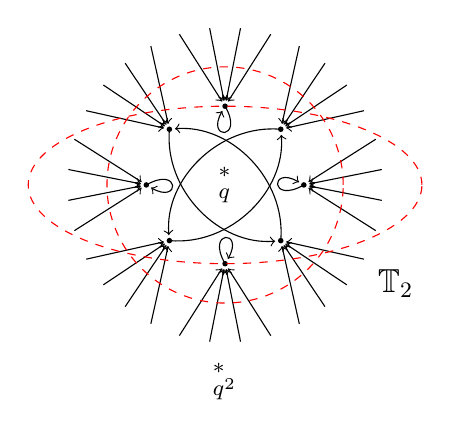
\begin{tikzpicture}[shorten >=2pt]
        \uncover<1-2>{\draw (0:0) node {\alert{\large$\FF_q^\ast$}};}
        \foreach \i in {0,...,7} {
          \pgfmathparse{int(2+!mod(\i,4))}
          \let\stop\pgfmathresult

          \uncover<1-\stop>{\fill (\i*45:1) circle (1pt);}

          \uncover<2-\stop>{
            \foreach \j in {0,...,3} {
              \draw[->] (\i*45-16.875+\j*11.25:2) -- (\i*45:1);
            }
          }
        }

        \foreach \i in {0,...,3} {
          \pgfmathparse{int(2+!mod(\i,2))}
          \let\stop\pgfmathresult

          \uncover<1-2>{
            \draw[->,bend right=50] (\i*90+45:1) to (\i*90+225:1);
          }
          \uncover<1-\stop>{
            \draw[->,in=\i*90+180-30,out=\i*90+180+30,loop] (\i*90:1) to ();
          }
        }

        \uncover<2>{
          \draw[dashed,red] (0:0) circle (1.5);
        }
        \uncover<2>{
          \draw (-90:2.5) node {\large\alert{$\FF_{q^2}^\ast$}};
        }
        \uncover<3->{
          \draw[dashed,red] (0:0) circle [x radius=2.5, y radius=1];
          \draw (-30:2.5) node {\large\alert{$\mathbb{T}_2$}};
        }
      \end{tikzpicture}
    \end{column}
    \begin{column}{0.5\textwidth}
      \begin{itemize}
      \item<1-> $\phi|_{\FF_q^\ast}$ bijective;
      \item<2-> $\phi|_{\FF_{q^2}^\ast}$ non surjective;
      \item<3-> $\mathbb{T}_2\subset\FF_{q^2}^\ast$ \emph{algebraic torus} of
        cardinality $q+1$.
      \end{itemize}
    \end{column}
  \end{columns}

  \begin{block}{}<3>
    \[\mathbb{T}_n(k) \cong
    \{\alpha\in L^\ast \;|\; \Norm_{L/F}(\alpha) = 1 \text{ for all } k\subset F\subsetneq L \}.\]
  \end{block}
\end{frame}

% ###################################################

\begin{frame}
  \frametitle{Towers from algebraic tori (Pell conics)}

  \begin{itemize}
  \item By Weil descent, $\mathbb{T}_2$ is isomorphic to a
    \emph{Pell conic};
  \item Multiplication in $\clot\FF_q$ induces a group law on
    the points.
  \end{itemize}
  
  \tikzset{
    point style/.style={circle, inner sep=0.9pt, fill = blue},
    extended line/.style={shorten >= -5mm, shorten <= -5mm}
  }

  \begin{center}
    \begin{tikzpicture}[scale = 0.9, every node/.style={scale=0.9}]
      \draw[name path = pellconic] (-1.5, 2.25) parabola bend (0, 0) (2.1, 4.41);
      \draw[style=help lines] (-1.7, 0) grid (2.2,4.5);
      % -----------
      \coordinate (N) at (1.3, 1.69);
      \coordinate (P) at (1.7, 2.89);
      \coordinate (Q) at (-1.3, 1.69);
      \coordinate (PQtemp) at ($(Q) + (N) - (P)$);
      % -----------
      \draw[extended line] (P)--(Q);
      \path[name path = pline] (PQtemp)--(N);
      \path [name intersections={of = pellconic and pline}];
      \coordinate (PQ) at (intersection-1);
      \draw [extended line] (N) -- (PQ);
      % -----------	
      \node[point style, fill = red, label=below right:$N$] at (N) {};
      \node[point style, label=below right:$P$] at (P) {};
      \node[point style, label=below left:$Q$] at (Q) {};
      \node[point style, label=below left:$P + Q$] at (PQ) {};

      \node[right = 4mm of current bounding box, text width = 7cm, fill = red!10, rounded corners, font = \small] (explain) {
        \alert{\it Pell conic:}
        \begin{equation*}
          \label{eq:Pell}
          C \;:\; x^2 - \Delta y^2 = 4
        \end{equation*}
        
        \vspace*{1cm}
        \textcolor{red}{Addition:} For $P=(x_1,y_1)$ and $Q=(x_2,y_2)$,
        \begin{equation*}
          P\oplus Q = \left(\frac{x_1x_2 + \Delta y_1y_2}{2},\; \frac{x_1y_2 + x_2y_1}{2}\right)
        \end{equation*}
      };
    \end{tikzpicture}	
  \end{center}
\end{frame}

% ###################################################

\begin{frame}
  \frametitle{Towers from algebraic tori}

  \begin{itemize}
  \item $\mathbb{T}_2 \to$ Pell conic $C$,
  \item multiplication in $\FF_{q^2} \to$ addition in $C$,
  \item $\ell$-th power $\to$ scalar multiplication $[\ell]$.
  \end{itemize}
  
  \begin{lemma}
    The abscissa of $[n]P$ is given by $C_n(x_1)$, where
    $C_n\in\ZZ[X]$ is the $n$-th \alert{Chebyshev
      polynomial}.
  \end{lemma}
  
  \begin{theorem}
    Let $P$ be a point not in $\ell C$, then we can compute
    \begin{equation*}
      Q_i(X_i) = C_{\ell^i}(X_i) - x_P
      \quad\text{and}\quad
      \alert{T_i(X_i) = C_{\ell}(X_i) - X_{i-1}}
    \end{equation*}
    using $O(\ell^i)$ operations.
  \end{theorem}
\end{frame}

% ###################################################

\begin{frame}[fragile]
  \frametitle{Towers from elliptic curves}

  \begin{itemize}
  \item \alert{Problem 1:} there is essentially one conic; we
    would like to have more group choices, \alert{elliptic
      curves} are an option.
  \item \alert{Problem 2:} $\ell$-multiplication on elliptic
    curves is a degree $\ell^2$ map; we must consider
    \alert{separable isogenies} instead.
  \end{itemize}
  
  \newcommand{\EC}[1]{{\color{blue} \ensuremath{E_{#1}}}}
  \newcommand{\IS}[1]{{\color{red} \ensuremath{\phi_{#1}}}}
  
  \begin{equation*}
    E_0 \;:\; y^2 = x^3 + ax + b, \quad a, b \in\FF_q,  \quad \ell \nmid (q-1), \quad \ell \mid \#E_0(\FF_q)
  \end{equation*}

  \begin{center}
    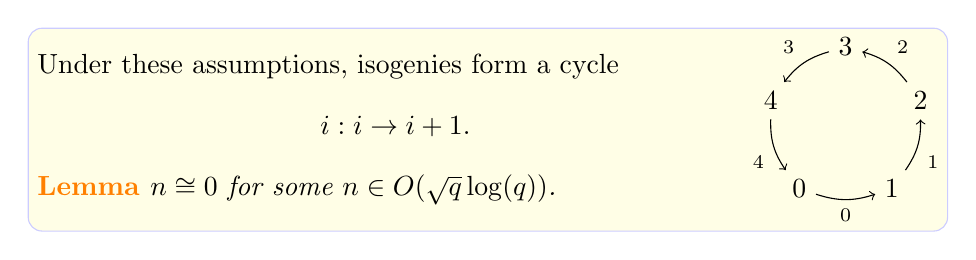
\begin{tikzpicture}
      \def\n{4}
      \foreach \i in {0,...,\n} {
        \pgfmathparse{360/(\n+1)*(\i-1/2) - 90}
        \let\angle\pgfmathresult
        \draw (\angle:1) node (E\i) {\EC{\i}};
        % \draw (\angle:0.4) node {\scriptsize$H_\i$};
        % \draw (\angle:0.7) node[rotate=\angle] {\scriptsize$\subset$};
      }
      \foreach \i in {0,...,\n} {
        \pgfmathparse{int(mod(\i+1, \n+1))}
        \let\j\pgfmathresult
        \draw (E\i) edge[->,bend right=18] node[auto, swap] {\scriptsize \IS{\i}} (E\j);
      }

      \node[left = -2.5mm of current bounding box.west] (explain) {
        \begin{minipage}{0.75\textwidth}
          Under these assumptions, isogenies form a cycle
          \[\IS{i}:\EC{i} \to \EC{i + 1}.\]

          \textbf{\color{orange} Lemma }{\it
            $\EC{n} \cong \EC{0}$ for some $n \in O(\sqrt{q}\log (q))$.}
        \end{minipage}
      };
      \begin{pgfonlayer}{background}
        \path[fill=yellow!10, rounded corners = 5pt, draw = blue!20] (current bounding box.south west) rectangle
        (current bounding box.north east);
      \end{pgfonlayer}
    \end{tikzpicture}
  \end{center}
\end{frame}

% ###################################################

\begin{frame}
  \frametitle{Towers from elliptic curves}
  
  \begin{lemma}[Couveignes and Lercier, 2011]
    Let $P \not\in \ell E_i$, and $\psi=\phi_{i-1}\circ\phi_{i-2}\circ\cdots\circ\phi_{j}$,\\
    then $\psi^{-1}(P)$ is irreducible of cardinality $\ell^{i-j}$.
  \end{lemma}

  \begin{block}{V\'elu's formulas}
    \begin{equation*}
      \begin{array}{crcl}
        \phi_i: & E_i &\longrightarrow & E_{i+1},\\
        & (x,y) &\longmapsto & \left(\frac{f_i(x)}{g_i(x)}, y\left(\frac{f_i(x)}{g_i(x)}\right)'\right),
      \end{array}
    \end{equation*}
  \end{block}
  
  \begin{block}{The $\ell$-adic tower}
    \begin{align*}
      T_1 &= f_{-1}(X_1) - \eta g_{-1}(X_1),\\ 
      \alert{T_i} &\alert{= f_{-i}(X_i) - X_{i-1} g_{-i}(X_i)}.
    \end{align*}
  \end{block}
\end{frame}

% **********************************************************
% **********************************************************

\section{Evaluating embeddings}

\begin{frame}
  \frametitle{\insertsection}
  
  \begin{block}{Observation}
    In all previous cases, from the form of $T_i$ we deduce
    \[X_{i-1} = f(X_i)/g(X_i)\]
    for some $f$ and $g$.  
    Going from multivariate to univariate is
    \[\sum a_j \alert{X_{i-1}^{\alpha_j}} X_i^{\beta_j} \mapsto
    \sum a_j \alert{\frac{f(X_i)^{\alpha_j}}{g(X_i)^{\alpha_j}}} X_i^{\beta_j} \]
  \end{block}
  
  \begin{definition}
    Let $P \in \FF_q[X,Y]$ and $n \in \NN$, with $\deg(P,X)< n$. Define
    $$P[f,g,n] = g^{n-1} P\left (\frac fg, Y\right) \in \FF_q[Y].$$
  \end{definition}
\end{frame}

% ###################################################

\begin{frame}
  \frametitle{Lifting: Multivariate $\to$ Univariate}
  
  \small
  \begin{center}
    \begin{tikzpicture}[every node/.style={scale=0.7}]
      \node [fill = red!10, draw = red!80]{
        \begin{minipage}{0.95\textwidth}
          \begin{algorithm}[H]
            \caption{Compose}
            \label{alg:compose}
            \begin{algorithmic}[1]
              \REQUIRE $P\in \FF_q[X,Y]$, $f,g\in \FF_q[Y]$, $n\in\NN$
              \IF {$n = 1$} 
              \RETURN $P$
              \ELSE
              \STATE $m \la \lceil n/2\rceil$
              \STATE Let $P_0,P_1$ be such that $P = P_0 + X^mP_1$
              \STATE $Q_0 \la$ Compose($P_0, f, g, m$)
              \STATE $Q_1 \la$ Compose($P_1, f, g, n-m$)
              \STATE $Q \la Q_0g^{n-m} + Q_1f^m$  \label{alg:compose:res}
              \RETURN $Q$
              \ENDIF
            \end{algorithmic}
          \end{algorithm}
        \end{minipage}
      };
    \end{tikzpicture}
  \end{center}
  
  \begin{theorem}
    \label{th:compose}
    Algorithm~\ref{alg:compose} computes $Q=P[f,g,n]$ using $O(\Mult(\ell
    n)\log(n))$ operations in $\FF_q$.
  \end{theorem}
\end{frame}

% ###################################################

\begin{frame}
  \frametitle{Pushing: Univariate $\to$ Multivariate}
  
  \small
  \begin{center}
    \begin{tikzpicture}[every node/.style={scale=0.7}]
      \node [fill = red!10, draw = red!80]{
        \begin{minipage}{0.95\textwidth}
          \begin{algorithm}[H]
            \caption{Decompose}
            \label{alg:decompose}
            \begin{algorithmic}[1]
              \REQUIRE $Q,f,g,h\in \FF_q[Y]$, $n \in \NN$ 
              \IF {$n=1$} 
              \RETURN $Q$
              \ELSE 
              \STATE $m \la \lceil n/2 \rceil$ 
              \STATE $u \la 1/ g^{n-m}\bmod f^m$ \label{alg:decompose:xgcd} 
              \STATE $Q_0 \la Q u \bmod f^m$ 
              \STATE $Q_1 \la (Q-Q_0 g^{n-m}) {\rm~div~} f^m$ 
              \STATE $P_0 \la$ Decompose($Q_0, f, g, h, m$) 
              \STATE $P_1 \la$ Decompose($Q_1, f, g, h, n-m$) 
              \RETURN $P_0 + X^m P_1$ 
              \ENDIF
            \end{algorithmic}
          \end{algorithm}
        \end{minipage}
      };
    \end{tikzpicture}
  \end{center}
  
  \begin{theorem}
    Algorithm~\ref{alg:decompose} computes a polynomial $P\in \FF_q[X,Y]$
    such that $Q=P[f,g,n]$ using
    $O(\Mult(\ell n)\log(n))$ operations in $\FF_q$.
  \end{theorem}
\end{frame}

% **********************************************************
% **********************************************************

\section{Implementation}

\begin{frame}
  \frametitle{\insertsection}
  
  \begin{center}
    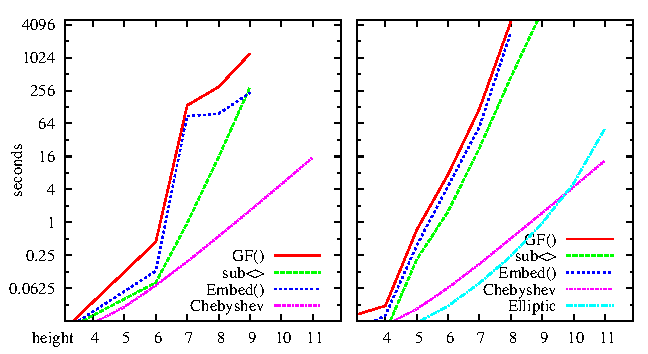
\includegraphics[width=9cm]{creat}\\\vspace*{1mm}
    \parbox{7cm}{\scriptsize Times for building $3$-adic towers on top of $\FF_2$ (left)
      and $\FF_5$ (right), in Magma (first three lines) and using our code.}
  \end{center}
  
  \begin{itemize}
    \small
  \item Intel Xeon E5620 clocked at 2.4 GHz, using Sage 5.5 and Magma 2.18.12
  \item Source code at \url{https://github.com/defeo/towers}.
  \end{itemize}
\end{frame}

%%

\section{Lattices (work in progress)}
\frame{\sectionpage}

%%

\begin{frame}
  \frametitle{Composita of fields}

  \begin{description}
  \item[Input:] \alert{$\FF_{p^m}=\FF_{p}[X]/P(X)$} and
    \alert{$\FF_{p^m}=\FF_{p}[Y]/P(Y)$}, with $(m,n)=1$.
  \item[Output:] \alert{$\FF_{p^{mn}}=\FF_{p}[Z]/R(Z)$}.
  \end{description}

  \begin{theorem}[Bostan \& Schost]
    Let \emph{$x,y$} be roots of \emph{$P,Q$}. 
    \begin{itemize}
    \item Both $xy$ and $x+y$ generate $\FF_{p^{mn}}$;
    \item The minimal polynomial of $xy$ or $x+y$ can be computed in
      \alert{$\tildO(mn)$}.
    \end{itemize}
  \end{theorem}
\end{frame}

%%

\begin{frame}
  \frametitle{Towards quasi-optimal embeddings}

  \begin{block}{Work in progress (with Doliskani and Schost)}
    \begin{itemize}
    \item Evaluate the maps $\FF_{p^n}\hookrightarrow\FF_{p^{mn}}$; \hfill
      \alert{$\tildO(mn)$}
    \item Evaluate the sections; \hfill \alert{$\tildO(mn)$}
    \item Full pushing $\FF_{p^{mn}} \to \FF_{p^n}^m$. \hfill \alert{$\tildO(mn\min(m,n))$}
    \end{itemize}
  \end{block}

  \begin{block}{Techniques}
    \begin{itemize}
    \item Bostan \& Schost algorithm;
    \item Bivariate trace computations (following Rouiller);
    \item transposed algorithms (following Bostan, Salvy \& Schost).
    \end{itemize}
  \end{block}
\end{frame}

%%

\begin{frame}
  \frametitle{Summary}

  \begin{block}{Results}
    \begin{itemize}
    \item $\ell$-adic towers very efficient for some $\ell$;
    \item Asymptotically good for most small $\ell$;
    \item Composita also asymptotically good;
    \item Full performances yet to test.
    \end{itemize}
  \end{block}

  \begin{block}{Open questions}
    \begin{itemize}
    \item Large prime degree extensions;
    \item Quasi-optimal full push down in composita;
    \item Arbitrary finite field isomorphisms in proven/practical
      subquadratic time.
    \end{itemize}
  \end{block}
\end{frame}

\end{document}
